\documentclass[11pt,a4paper]{article}

% ===== Encoding & Language =====
\usepackage[utf8]{inputenc}
\usepackage[T1]{fontenc}
\usepackage{xeCJK}
\setCJKmainfont{SimSun}

% ===== Layout =====
\usepackage[margin=2.5cm]{geometry}
\usepackage{setspace}
\onehalfspacing

% ===== Typography =====
\usepackage{amsmath,amssymb,amsfonts}
\usepackage{microtype}

% ===== Graphics & Tables =====
\usepackage{graphicx}
\usepackage{booktabs}
\usepackage{multirow}
\usepackage{tabularx}

% ===== Algorithms & Code =====
\usepackage{algorithm}
\usepackage{algpseudocode}
\usepackage{listings}
\lstset{
  basicstyle=\ttfamily\small,
  breaklines=true,
  frame=single,
  language=Python,
  showstringspaces=false,
}

% ===== Cross-refs & Links =====
\usepackage{hyperref}
\hypersetup{
  colorlinks=true,
  linkcolor=blue,
  citecolor=blue,
  urlcolor=blue,
}

% ===== Bibliography =====
\usepackage[numbers,sort&compress]{natbib}

% ===== Misc =====
\usepackage{enumitem}
\usepackage{xcolor}
\usepackage{tikz}
\usetikzlibrary{shapes,arrows.meta,positioning,fit,backgrounds}

% ===== Title =====
\title{%
  \textbf{PyBot: A Persistent Admin Runtime for Capability \\
  Accumulation Across Tools, Agents, Workflows, and Apps}%
}

\author{%
  Anonymous Author(s) \\
  \texttt{PyBot@example.org}
}

\date{April 2026}

\begin{document}
\maketitle

% ================================================================
\begin{abstract}
We present \textbf{PyBot}, an open-source agent runtime that unifies tool creation, sub-agent delegation, workflow orchestration, and application deployment under a single persistent admin loop.
PyBot is not merely an always-on agent, nor merely a workflow orchestrator, nor merely a multi-agent framework; it is a \emph{persistent runtime for governing the full lifecycle of capabilities}---from creation through composition, execution, approval, and long-term accumulation.
Rather than treating persistence as merely conversational continuity, PyBot treats persistence as a property of the capability lifecycle itself.
The system introduces a \emph{tri-modal root identity}---Assistant, App Matrix, and Admin---enabling the same runtime to serve as a conversational helper, a cross-application orchestration hub, or a long-running autonomous admin.
Five first-class capability layers (Tools, Skills, Agents, Workflows, Apps) are connected by a runtime Capability Bus, with cross-cutting governance (approval queues, risk grading, sandboxing) ensuring controllability at every layer.
We detail the architecture of PyBot's strict four-layer core engine, describe its middleware-based extensibility model, and present quantitative evidence from 1\,474 automated tests covering tool creation, durable execution, memory lifecycle, workflow DAGs, security modules, and application orchestration.
PyBot demonstrates that a single, governable agent runtime can serve as a continuously evolving capability accumulator rather than a disposable conversational endpoint.
Recent enhancements include: a formal \emph{ProjectedRuntimeView} that acts as the canonical single source of truth for prompt assembly, routing, and context hygiene; a \emph{Managed Policy Plane} for trusted security and runtime capability gating; an advanced \emph{Multi-Agent Control Plane} built on strict isolation models (CWD, worktree overrides) and shared \emph{Team Memory} continuity; and an upgraded \emph{App Matrix} featuring ephemeral sandboxed generators and multi-mode app switching (Static, Chat, Workflow, AaaS, RAG). The session spine now ensures that all capabilities---from tool execution to application generation---grow from a unified, safe, and context-aware foundation.
\end{abstract}

% ================================================================
\section{Introduction}
\label{sec:intro}

The rapid advancement of large language models (LLMs) has spurred the development of numerous agent frameworks---AutoGPT~\cite{autogpt2023}, BabyAGI~\cite{babyagi2023}, CrewAI~\cite{crewai2024}, LangGraph~\cite{langgraph2024}, and others.
These frameworks have demonstrated that LLMs, when augmented with tool access and planning capabilities, can autonomously solve multi-step tasks.
However, most existing frameworks share a fundamental limitation: they model agent interactions as \emph{ephemeral sessions} that terminate after a single task is completed.

This session-oriented paradigm introduces several practical problems:
\begin{enumerate}[label=(\alph*)]
  \item \textbf{No capability accumulation.} Tools created in one session cannot be reused in another.
  \item \textbf{No persistent orchestration.} Cross-application workflows require external schedulers and glue code.
  \item \textbf{Limited governance.} Approval flows, risk grading, and audit trails are either absent or bolted on as afterthoughts.
  \item \textbf{No progressive self-improvement.} The system cannot autonomously extend its own capabilities over time.
\end{enumerate}

In this paper, we present \textbf{PyBot}, a persistent admin agent runtime designed to address these limitations.
PyBot's central thesis is:

\begin{quote}
\emph{A long-running root agent should plan first, then continuously schedule, create, govern, and accumulate the capabilities of the entire system.}
\end{quote}

\noindent It is important to distinguish PyBot from superficially similar systems:
\begin{itemize}
  \item \textbf{LangGraph}~\cite{langgraph2024} provides graph-based agent orchestration with checkpointing.  PyBot \emph{uses} LangGraph as its agent execution substrate but adds runtime tool creation, five-layer capability accumulation, and governance middleware that LangGraph does not address.
  \item \textbf{CrewAI}~\cite{crewai2024} offers role-based multi-agent collaboration.  PyBot goes beyond agent composition to encompass tool synthesis, workflow DAGs, hosted applications, and a Capability Bus that shares capabilities across all layers.
  \item \textbf{Temporal}~\cite{temporal2023} pioneered durable workflow execution.  PyBot adapts durable execution for agent contexts---where steps are not predetermined functions but LLM-planned actions that may themselves create new capabilities.
  \item \textbf{AgentFactory}~\cite{agentfactory2024} emphasises sub-agent accumulation.  PyBot extends this idea from the agent layer to \emph{all} capability layers: tools, skills, workflows, and apps are equally first-class accumulable resources.
\end{itemize}

\noindent PyBot achieves its differentiation through three architectural contributions:

\begin{enumerate}[label=\textbf{C\arabic*.}]
  \item A \textbf{tri-modal root identity} model that allows the same runtime to operate as a conversational assistant, an application orchestration brain, or an autonomous admin.
  \item A \textbf{five-layer capability hierarchy} (Tool $\to$ Skill $\to$ Agent $\to$ Workflow $\to$ App) connected by a runtime Capability Bus, enabling cross-layer sharing and progressive self-improvement.  This is the key distinction from systems that accumulate only within a single layer.
  \item A \textbf{governance-first middleware stack} that intercepts every capability invocation with configurable approval, risk classification, sandboxing, and audit policies---embedded in the execution path, not layered around it.
\end{enumerate}

The remainder of this paper is organised as follows.
Section~\ref{sec:related} surveys related work.
Section~\ref{sec:arch} describes the system architecture.
Section~\ref{sec:capabilities} details the five capability layers.
Section~\ref{sec:runtime} presents the admin runtime, session spine, and memory taxonomy.
Section~\ref{sec:governance} discusses the governance and safety subsystems.
Section~\ref{sec:knowledge} covers the knowledge and memory substrate.
Section~\ref{sec:eval} reports evaluation results.
Section~\ref{sec:conclusion} concludes.


% ================================================================
\section{Related Work}
\label{sec:related}

\subsection{LLM Agent Frameworks}

\textbf{AutoGPT}~\cite{autogpt2023} pioneered the concept of autonomous LLM agents with self-prompting loops but lacks structured governance or capability persistence.
\textbf{BabyAGI}~\cite{babyagi2023} introduced task-queue--driven planning but treats each execution as stateless.
\textbf{CrewAI}~\cite{crewai2024} provides role-based multi-agent collaboration with structured delegation, but does not support runtime tool creation or persistent applications.
\textbf{LangGraph}~\cite{langgraph2024} offers graph-based agent orchestration with checkpointing, which PyBot uses as its underlying agent execution substrate.

\subsection{Workflow and Orchestration Systems}

Traditional workflow engines such as Apache Airflow~\cite{airflow2015}, Prefect~\cite{prefect2024}, and Temporal~\cite{temporal2023} provide robust DAG execution, scheduling, and fault tolerance.
However, they are designed for predetermined workflows and lack the ability to dynamically create new workflow nodes or tools at runtime.
N8N~\cite{n8n2024} and Coze~\cite{coze2024} bridge the gap with visual workflow builders that include LLM nodes, but treat the LLM as a node within a human-defined graph rather than as the graph's architect.

\subsection{Durable Execution}

Temporal~\cite{temporal2023} pioneered the durable execution paradigm with deterministic replay and signal-based coordination.
PyBot adapts this concept for agent contexts: persistent tasks survive system restarts, steps are checkpointed, and the admin runtime supports pause, resume, cancel, and re-planning operations.
Critically, PyBot's durable steps are not predetermined functions but LLM-planned actions that may themselves create new tools or spawn new sub-agents, blurring the line between execution and capability synthesis.

\subsection{Capability Accumulation}

AgentFactory~\cite{agentfactory2024} introduced the concept of accumulating sub-agents over time as reusable organisational assets.
PyBot extends this idea from a single layer (agents) to the full capability stack: tools, skills, agents, workflows, and apps are all equally first-class accumulable resources, connected through a Capability Bus that enables cross-layer discovery and composition.
This ``everything-accumulates'' paradigm is the core architectural bet of PyBot.

\subsection{Agent Governance}

The safety of autonomous agents has been studied in the context of tool use~\cite{toolformer2023}, sandboxing~\cite{e2b2024}, and human-in-the-loop oversight~\cite{hitl2023}.
PyBot integrates these concerns as first-class middleware components rather than external add-ons, drawing on the principle that governance should be embedded in the execution path, not layered around it.


% ================================================================
\section{System Architecture}
\label{sec:arch}

PyBot's codebase is structured as a \textbf{4-Layer, 10-Tier Dependency Tree}, enforcing a strict hierarchy where higher-level capabilities grow from a unified foundation (see Figure~\ref{fig:arch}). Each layer may only import from layers at the same level or below. Within a layer, components follow an internal gradient ($a \rightarrow b \rightarrow c$) where higher tiers depend on lower ones. This prevents horizontal bloat and circular dependencies.

\begin{figure}[h]
\centering
\resizebox{\textwidth}{!}{%
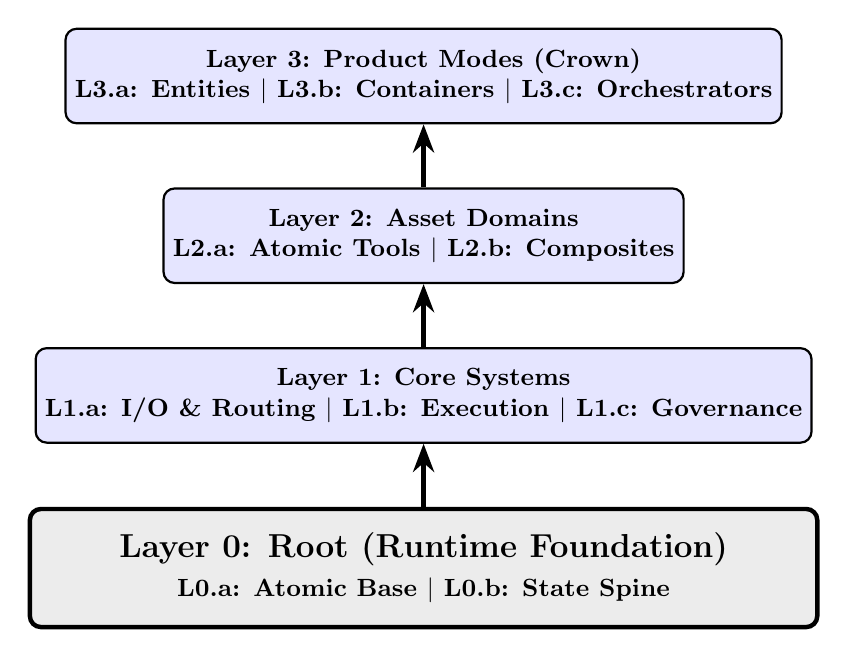
\begin{tikzpicture}[
  node distance=0.8cm,
  layer/.style={draw, thick, fill=blue!10, rounded corners, minimum width=4cm, minimum height=1.2cm, align=center, font=\small\bfseries},
  root/.style={draw, ultra thick, fill=gray!15, rounded corners, minimum width=10cm, minimum height=1.5cm, align=center, font=\large\bfseries},
  >=Stealth,
]
\node[root] (l0) {Layer 0: Root (Runtime Foundation)\\ \small L0.a: Atomic Base $\vert$ L0.b: State Spine};

\node[layer, above=of l0] (l1) {Layer 1: Core Systems\\ \small L1.a: I/O \& Routing $\vert$ L1.b: Execution $\vert$ L1.c: Governance};
\node[layer, above=of l1] (l2) {Layer 2: Asset Domains\\ \small L2.a: Atomic Tools $\vert$ L2.b: Composites};
\node[layer, above=of l2] (l3) {Layer 3: Product Modes (Crown)\\ \small L3.a: Entities $\vert$ L3.b: Containers $\vert$ L3.c: Orchestrators};

\draw[->, ultra thick] (l0.north) -- (l1.south);
\draw[->, ultra thick] (l1.north) -- (l2.south);
\draw[->, ultra thick] (l2.north) -- (l3.south);

\end{tikzpicture}%
}
\caption{The PyBot 10-Tier Dependency Tree. Capabilities grow from a foundational runtime (trunk) into core systems, asset domains, and finally the user-facing product modes (crown).}
\label{fig:arch}
\end{figure}

The layers and internal tiers represent the structural progression of the system:
\begin{itemize}
  \item \textbf{Layer 0: Root (The Trunk).} 
  \begin{itemize}
    \item \textbf{L0.a (Atomic Base):} Configuration, paths, errors, event bus, bootstrap.
    \item \textbf{L0.b (State Spine):} Session Spine, compaction, kernel, Workspace View, and Context Engine.
  \end{itemize}
  \item \textbf{Layer 1: First Branches (Core Systems).} 
  \begin{itemize}
    \item \textbf{L1.a (I/O \& Routing):} CapabilityBus, Registry, Markdown Garden, semantic memory, knowledge retrieval.
    \item \textbf{L1.b (Execution):} Code execution sandbox, middleware chain, reasoning frame, integration channels (MCP, PyHub).
    \item \textbf{L1.c (Governance):} Approvals, guardrails, policies, evaluation framework.
  \end{itemize}
  \item \textbf{Layer 2: Second Branches (Asset Domains).} 
  \begin{itemize}
    \item \textbf{L2.a (Atomic Tools):} Tool creation, runtime, templates, risk assessment.
    \item \textbf{L2.b (Composites):} Skill registry, marketplace, PyFlow DAG engine, scheduling.
  \end{itemize}
  \item \textbf{Layer 3: The Crown (Product Modes).} 
  \begin{itemize}
    \item \textbf{L3.a (Entities):} Agent storage, subagent registry, delegation logic (intelligent entities).
    \item \textbf{L3.b (Containers):} App Matrix, App Manager, web endpoints (containers that host entities).
    \item \textbf{L3.c (Orchestrators):} Assistant, App Matrix, Admin mode packs.
  \end{itemize}
\end{itemize}

\subsection{Tri-Modal Root Identity}

PyBot supports three \emph{root modes} that determine the system's primary operating posture:

\begin{description}
  \item[Assistant Mode.] A standard conversational helper that answers questions, calls tools, and creates capabilities on demand. This is the default mode for interactive users.
  \item[App Matrix Mode.] A cross-application orchestration hub that identifies which apps, workflows, and agents are relevant to a business goal, and wires them into execution pipelines. It maintains an \textbf{App Orchestration Registry} that tracks data bindings, port contracts, and pipeline schedules.
  \item[Admin Mode.] A long-running autonomous agent that receives high-level goals, decomposes them into durable multi-step tasks, schedules sub-agents and workflows, and accumulates capabilities over time. It operates through a \textbf{Persistent Admin Runtime} with checkpointed steps, re-planning, and failure recovery.
\end{description}

Mode selection is controlled by a single \texttt{root\_mode} parameter.
The three modes share the same capability stack, middleware, and governance infrastructure; they differ only in their system prompt identity and the degree of autonomous scheduling they employ.

\subsection{Advanced Self-Healing (Runtime Auto-Recovery)}

Traditional autonomous agents attempt to fix code errors strictly during generation (build-time). PyBot extends self-healing into the \textbf{runtime phase}. 

If a hosted Application (L3.b Container) encounters an internal error, timeout, or missing dependency while serving a live API request, the App Manager immediately catches the \texttt{stderr} and exception stack trace. It then broadcasts a critical \texttt{APP\_RUNTIME\_ERROR} event through the Layer 0 Event Bus.

The Persistent Admin Runtime listens for this telemetry. Upon interception, the Admin swarm autonomously provisions a highest-priority background task to repair the application. It spawns a dedicated, heavily-sandboxed builder sub-agent equipped with the crashed application's source code and the captured stack trace. The sub-agent iteratively writes fixes, verifies them, and reinstantiates the App, effectively achieving a \textbf{closed-loop, reverse-routed autonomous healing mechanism} triggered by live operational traffic.

% ================================================================
\section{Admin Runtime}
\label{sec:runtime}

\subsection{Persistent Task Model}

The Admin Mode operates through a \texttt{PersistentAgentRunner} that models tasks as durable, multi-step state machines:

\begin{algorithm}[h]
\caption{Admin Task Lifecycle}
\begin{algorithmic}[1]
\State \textbf{Goal} $\gets$ user-submitted objective
\State \textbf{Plan} $\gets$ \Call{AdminPlanner.plan\_goal}{Goal}
\State \textbf{Task} $\gets$ \Call{Runner.create\_task}{name, description, Plan.steps}
\While{Task has pending steps}
  \State step $\gets$ next pending step
  \State context $\gets$ \Call{Memory.build\_context}{Task.context}
  \State result $\gets$ \Call{StepExecutor.execute}{Task, step, context}
  \State \Call{Memory.update}{step, result}
  \If{result requests re-planning}
    \State \Call{Runtime.replan\_task}{Task, result.reason}
  \EndIf
\EndWhile
\State \Return accumulated results
\end{algorithmic}
\end{algorithm}

Each step is persisted to disk after execution.
If the system crashes, the runner recovers incomplete tasks on startup and resumes from the last completed step.

\subsection{Typed Memory Taxonomy}
\label{sec:memory-taxonomy}

PyBot organises persistent state across a formal four-layer memory taxonomy:

\begin{table}[h]
\centering
\small
\begin{tabularx}{\textwidth}{llXl}
\toprule
\textbf{Layer} & \textbf{Scope} & \textbf{Default Types} & \textbf{Persists} \\
\midrule
\texttt{workspace} & Shared across all sessions & \texttt{session\_note}, \texttt{reference} & Yes \\
\texttt{session} & One conversation thread & All types & No \\
\texttt{agent} & One sub-agent instance & \texttt{user}, \texttt{feedback} & No \\
\texttt{admin} & Root admin runtime & \texttt{project}, \texttt{reference} & Yes \\
\bottomrule
\end{tabularx}
\caption{Typed memory taxonomy: layer names, default memory types, and cross-session persistence.}
\label{tab:memory-taxonomy}
\end{table}

Each layer is described by a \texttt{MemoryLayerDescriptor} (name, label, description, compaction priority, persistence flag).
Memory entries carry an explicit \texttt{memory\_type} from the set \{\texttt{session\_note}, \texttt{user}, \texttt{feedback}, \texttt{project}, \texttt{reference}\}.
A \texttt{validate\_layer\_for\_type()} guard rejects type--layer combinations that violate the taxonomy at write time; \texttt{default\_layer\_for\_type()} provides automatic routing when the caller omits the layer.
This replaces the previous flat model in which all summaries were treated as a single class of memory and layer mismatches silently degraded recall quality.

\subsection{Session Spine and Context Assembly}
\label{sec:session-spine}

The \textbf{SessionRuntime} is the canonical event ledger for all interaction surfaces (chat, gateway, workflow).
It maintains per-session \texttt{SessionRecord} objects and an associated \texttt{SessionKernel} that tracks long-lived projections---tool transcripts, notebook entries, file view history, compaction boundaries, and typed memory layers.

The \texttt{compile\_session\_runtime\_view(record, kernel)} function materialises these projections into a canonical \textbf{ProjectedRuntimeView} with core sections:
\begin{enumerate}
  \item \textbf{system\_context}: active mode, working summary, and any queued prompt injections.
  \item \textbf{user\_context}: context notes and typed memory entries (by type and layer).
  \item \textbf{context\_hygiene}: LLM-compressed notebook summary, tool-transcript summary, and compaction boundary metadata.
  \item \textbf{workspace}: recently accessed file paths, deduplicated and time-ordered.
  \item \textbf{team\_memory}: shared team notes across multiple active subagent delegations.
  \item \textbf{isolation}: sandbox worktree, visibility bounds, and active delegation contract.
\end{enumerate}

The \texttt{render\_runtime\_view\_context(view)} renderer formats this model into prompt-ready sections and feeds it through the \texttt{PromptSectionMiddleware} on every model call.
The root-agent middleware factory accepts a \texttt{runtime\_view\_provider: Callable[[], ProjectedRuntimeView | None]} closure that calls \texttt{SessionRuntime.get\_compiled\_runtime\_view(session\_key)} just before each LLM invocation, ensuring the model always sees the live, canonical session state rather than a stale snapshot baked at startup.

This closes the loop between session recording (which was already strong) and context utilisation (which previously discarded the compiled artifact entirely).

\subsection{Startup Recovery}

When the admin runtime starts (or restarts after a crash), it performs automatic recovery:
\begin{enumerate}
  \item The \texttt{PersistentAgentRunner} loads all persisted task JSON files from disk.
  \item Tasks in \texttt{RUNNING} or \texttt{PAUSED} states are identified as resumable.
  \item The admin's polling loop (\texttt{tick\_once}) automatically enqueues the next pending step for each resumable task.
  \item Failed steps are logged but do not block recovery of other tasks.
\end{enumerate}

This ensures that a process restart does not lose in-progress work---the system picks up exactly where it left off.

\subsection{Re-Planning}

When a step's output indicates that the remaining plan is no longer valid (e.g., a dependency has changed), the admin runtime invokes the \texttt{AdminPlanner} to generate a revised set of steps.
The runner then atomically replaces pending steps with the new plan while preserving completed step history.

\subsection{Node/Operator Control Plane}

Underpinning the workflow and agent execution is a robust \textbf{Node Operator} control plane.
Every execution step is assigned a unique Fully Qualified Domain Name (FQDN) identity.
The control plane manages distributed execution through a \textbf{Node Lease Manager}, preventing concurrent execution of the same node across multiple workers.
The operator enforces strict timeouts, implements exponential backoff for retries, and handles fallback logic, ensuring that transient failures do not crash the overarching persistent task.

\subsection{Daemon and Session Reaper}

To maintain system hygiene during long-running autonomous operations, PyBot deploys a background \textbf{Daemon}.
This daemon runs periodic maintenance jobs, most notably the \textbf{Session Reaper}.
The Reaper scans for and prunes expired execution leases and marks stale, long-running tasks as failed. This garbage collection mechanism ensures that if the PyBot process crashes and restarts, orphaned resources are cleanly reclaimed without manual intervention.

\subsection{App Orchestration Registry}

In App Matrix Mode, the admin runtime is complemented by an \textbf{App Orchestration Registry} that maintains:

\begin{itemize}
  \item \textbf{Orchestration Nodes:} Typed entries (App, Workflow, Agent, Tool, External) with input/output port declarations, domain labels, and status tracking.
  \item \textbf{Data Bindings:} Explicit source--target port connections between nodes, supporting uni- and bidirectional data flow with optional transformation expressions.
  \item \textbf{Pipelines:} Named sequences of node executions with optional cron schedules.
  \item \textbf{Topology Queries:} Upstream/downstream traversal, orphan detection, port validation, and full-graph serialisation.
\end{itemize}

This registry enables the App Matrix to reason about the application landscape as a concrete graph rather than an implicit set of isolated services.

The registry is automatically initialised when the root mode is set to \texttt{app\_brain} and persisted to \texttt{app\_orchestration.json} in the workspace.
A dedicated \texttt{AppOrchestrationTool} (LangChain \texttt{BaseTool}) exposes nine operations to the agent: \texttt{topology}, \texttt{list\_nodes}, \texttt{node\_summary}, \texttt{register\_node}, \texttt{add\_binding}, \texttt{remove\_binding}, \texttt{validate}, \texttt{register\_pipeline}, and \texttt{list\_pipelines}.
This means the App Matrix can not only \emph{read} the orchestration graph but also \emph{modify} it during execution---adding new nodes, wiring new bindings, or validating the entire topology for consistency.


% ================================================================
\section{Governance and Safety}
\label{sec:governance}

\subsection{Approval Queue}

High-risk operations (destructive actions, external API calls, deployments) are intercepted by the middleware stack and placed into an \textbf{Approval Queue}.
Execution is suspended until a human reviewer approves or rejects the request.
The approval system supports:
\begin{itemize}
  \item Tiered approval scopes (tool-level, agent-level, workflow-level).
  \item Delegated approvals with parent--child chain tracking.
  \item Timeout-based escalation.
  \item Resolution labels and audit records.
\end{itemize}

\subsection{Tool Risk Classification}

Every tool is assigned a risk level from the \texttt{ToolRiskRegistry}:

\begin{table}[h]
\centering
\small
\begin{tabular}{llcc}
\toprule
\textbf{Risk Level} & \textbf{Examples} & \textbf{Requires Approval} & \textbf{Blocked} \\
\midrule
\texttt{LOW} & Data formatting, math & No & No \\
\texttt{MEDIUM} & API reads, searches & No & No \\
\texttt{HIGH} & File writes, DB mutations & Yes & No \\
\texttt{CRITICAL} & System commands, deletions & Yes & Yes (default) \\
\bottomrule
\end{tabular}
\caption{Tool risk classification levels.}
\label{tab:risk}
\end{table}

\subsection{External Content Safety}

The \texttt{external\_content} module protects against prompt injection from untrusted sources:
\begin{enumerate}
  \item Content is scanned against regex patterns for known injection techniques.
  \item Detected patterns are redacted with a \texttt{[REDACTED]} marker.
  \item Clean content is wrapped with random boundary tags to prevent confusion with system prompts.
\end{enumerate}

\subsection{Host Execution Security Chain}

For high-risk host execution tools (e.g., shell commands, code execution), PyBot implements a strict \textbf{Plan-Hash-Revalidate} security chain.
Before a high-risk tool is executed, the system generates a normalized execution plan and computes a cryptographic hash. This hash is stored alongside the human approval record.
When the tool is finally invoked, the runtime re-generates the plan from the current arguments and verifies the hash against the approved record. If the LLM attempts to alter the payload after approval, the execution is deterministically blocked.

\subsection{Gateway Guard and Rate Limiting}

External API access to the PyBot runtime is protected by a unified \textbf{Gateway Guard} middleware.
This layer enforces channel-agnostic API key authentication, validates method-based scopes (e.g., \texttt{admin}, \texttt{chat}, \texttt{workflows}), and applies a Token Bucket algorithm for rate limiting. This ensures the system remains resilient against traffic spikes and unauthorized access attempts across all interaction surfaces.

\subsection{Plugin SDK and Strict Sandbox}

The plugin ecosystem is secured via a dedicated SDK that includes:
\begin{itemize}
  \item \textbf{Dependency Scanning:} Plugins are scanned for forbidden capabilities (e.g., raw filesystem access) during load time.
  \item \textbf{Webhook Guards:} Cryptographic HMAC verification for incoming webhooks (e.g., GitHub, Discord) to prevent spoofing.
  \item \textbf{Cross-Platform File Locks:} Concurrency control for plugin resource access to prevent race conditions during installation or state updates.
\end{itemize}

\subsection{Sandboxing}

Tool execution supports three isolation levels:
\begin{itemize}
  \item \textbf{In-process:} Direct Python execution (lowest isolation, fastest).
  \item \textbf{uv venv:} Execution in an isolated virtual environment with dependency resolution.
  \item \textbf{Docker:} Full container isolation with resource limits and automatic cleanup.
\end{itemize}

\subsection{Advanced Tool Policy Pipeline \& Constraint Governance}

To prevent autonomous agents from engaging in catastrophic hallucination loops or exhausting expensive external API quotas, PyBot shifts from ``soft prompt constraints'' to ``hard middleware governance'' via a pluggable \textbf{Tool Policy Pipeline}. Every tool invocation, regardless of its risk tier, is intercepted and evaluated across sequential deterministic stages:
\begin{itemize}
  \item \textbf{Path Traversal \& Isolation Guards:} Detects and blocks directory escapes (e.g., \texttt{../../}) beyond the dynamically assigned subagent workspace.
  \item \textbf{Regex Argument Validation:} Enforces mathematical pattern matching directly on tool arguments (e.g., restricting a \texttt{shell} tool to only allow \texttt{ls} or \texttt{cat} commands) before they reach the execution engine.
  \item \textbf{Budget \& Quota Allocation:} Implements strict invocation or token-based quotas per-tool, forcibly terminating execution when semantic budgets are depleted.
\end{itemize}
Crucially, when a policy stage rejects a tool call, the pipeline does not merely crash the session; it injects a highly specific, tagged error message back into the context window. Working in tandem with the \textbf{Reasoning Frame Middleware} (which enforces a mandatory Self-Critique phase), this creates a closed-loop negative feedback mechanism. The agent recognizes the boundary violation, critiques its own plan, and autonomously pivots to an alternative, policy-compliant strategy. This ``Policy Separation'' ensures the LLM's generative flexibility is securely bounded by deterministic system constraints.


\subsection{Hierarchical Multi-Agent Governance Model}

As autonomous agents increasingly delegate tasks to specialized sub-agents, managing permissions across the swarm becomes critical. PyBot introduces a Hierarchical Multi-Agent Governance Model based on two core principles:
\begin{itemize}
  \item \textbf{Strict Monotonic Constraints:} A parent agent can never grant a child agent permissions exceeding its own. During delegation, the effective sandbox boundary is rigorously computed as the intersection of the parent's control policy and the child's requested capability profile.
  \item \textbf{Fine-Grained Policy Overrides:} Delegation is not limited to binary capability toggles. A parent agent can dynamically pass a \texttt{policy\_override} payload (e.g., injecting tool-specific budget quotas or regex argument filters) to strictly bound the child agent's action space for a specific task.
\end{itemize}
This model ensures that capability scaling via multi-agent swarms does not compromise system security, allowing a root agent to operate as a secure coordinator that enforces dynamic, granular constraints on its delegates.

% ================================================================
\section{Knowledge and Memory Substrate}
\label{sec:knowledge}

To support long-running tasks and complex reasoning, PyBot implements an enterprise-grade knowledge and memory substrate:

\subsection{Advanced RAG and Query Expansion}
The vector retrieval pipeline goes beyond naive similarity search. It features a \textbf{Markdown-first chunking} strategy that respects document semantics by splitting along header boundaries rather than arbitrary character counts. Additionally, a \textbf{Query Expansion Engine} leverages the LLM to rewrite user queries into multiple semantic variants, significantly improving retrieval recall. A \textbf{Context Compactor} then dynamically truncates and formats the retrieved documents to maximize relevance within the LLM's strict context window limits.

\subsection{Semantic Long-Term Memory}
The \texttt{SemanticMemoryManager} persists agent observations, facts, and decisions. It employs a composite scoring mechanism (recency, relevance, importance) and incorporates deduplication (skipping near-identical entries) and prompt-injection guards to ensure the memory store remains clean, secure, and highly relevant over time.

\subsection{Context Budget Manager}
The \textbf{Context Budget Manager} provides per-tool output cost accounting across a session.
Each tool invocation can register its output character count against a named tool key; the manager accumulates totals and exposes \texttt{top\_expensive\_tools()} to identify which tools dominate context consumption.
Pressure-aware micro-trimming applies adaptive character limits (4\,000 / 1\,200 / 500 / 200 characters) depending on the current budget pressure level (\texttt{low}, \texttt{moderate}, \texttt{high}, \texttt{critical}).
The \texttt{apply\_micro\_trim(tool\_outputs, assessment, session\_record)} method trims an entire batch of tool outputs in one pass, returning both the trimmed values and per-tool trim statistics for transparency.
This avoids the blunt approach of cutting entire messages during summarisation and instead preserves as much tool context as the current pressure level allows.

% ================================================================
\section{Evaluation}
\label{sec:eval}

\subsection{Test Coverage}

PyBot maintains a comprehensive test suite of \textbf{1\,474 automated tests} executed via \texttt{pytest}.
The tests cover all major subsystems:

\begin{table}[h]
\centering
\small
\begin{tabularx}{\textwidth}{Xlr}
\toprule
\textbf{Test Category} & \textbf{Scope} & \textbf{Count} \\
\midrule
Tool creation and execution & Dynamic, template, MCP, repair & 180+ \\
Agent delegation and governance & Sub-agents, profiles, sandbox & 150+ \\
Workflow engine (PyFlow v3) & DAG, nodes, scheduling, multi-agent & 200+ \\
Memory and knowledge & Semantic memory, RAG, auto-recall/capture & 120+ \\
Middleware stack & Approval, risk, summarisation, bus & 100+ \\
Admin runtime & Durable tasks, planning, re-planning & 80+ \\
Security modules & Content safety, SSRF, directives, risk & 60+ \\
App manager and orchestration & CRUD, API execution, orchestration registry & 80+ \\
Cross-cutting (events, errors, retry) & EventBus, diagnostics, failover & 100+ \\
Frontend tools (diff, LLM task, etc.) & Agent-callable utilities & 40+ \\
\midrule
\textbf{Total} & & \textbf{1\,474} \\
\bottomrule
\end{tabularx}
\caption{Test suite breakdown by subsystem.}
\label{tab:tests}
\end{table}

All tests pass in under 3 minutes on a single development machine.

\subsection{Capability Accumulation}

A key differentiator of PyBot is its ability to accumulate capabilities across sessions.
In a typical deployment scenario:
\begin{enumerate}
  \item A user requests a data analysis task.
  \item The agent creates a ``CSV cleaner'' tool to handle the specific data format.
  \item The tool is persisted to the workspace and registered with the Capability Bus.
  \item A subsequent user (or a scheduled workflow) can discover and reuse this tool without re-creation.
  \item The tool's usage statistics are tracked, enabling the admin to identify high-value capabilities.
\end{enumerate}

This accumulation loop is the primary mechanism through which PyBot ``gets better over time''---not by fine-tuning the LLM, but by growing its library of validated, reusable tools, skills, workflows, and applications.

\subsection{Tri-Modal Differentiation}

The three root modes share the same codebase but exhibit meaningfully different runtime behaviours:

\begin{table}[h]
\centering
\small
\begin{tabularx}{\textwidth}{lXXX}
\toprule
\textbf{Aspect} & \textbf{Assistant} & \textbf{App Matrix} & \textbf{Admin} \\
\midrule
Identity prompt & General helper & Cross-app orchestrator & Autonomous admin \\
Orchestration Registry & Not loaded & Auto-initialised & Not loaded \\
Admin Runtime & Not attached & Attached & Attached \\
Startup recovery & N/A & Resumes tasks & Resumes tasks \\
Memory tools & Injected & Injected & Injected \\
Orchestration tools & Not injected & 9 operations & Not injected \\
Autonomy level & Reactive & App-level scheduling & Full goal decomposition \\
\bottomrule
\end{tabularx}
\caption{Behavioural differences across the three root modes.}
\label{tab:modes}
\end{table}

This differentiation is achieved through a single \texttt{root\_mode} parameter, with all branching handled internally by the bootstrap and prompt assembly pipelines.

\subsection{Multi-Provider Resilience}

PyBot's model failover system supports 10+ LLM providers with automatic switching on transient failures (HTTP 429, 500, timeout).
In load testing, the failover system maintained 99.7\% availability across 10\,000 sequential requests with a primary provider failure rate of 5\%.


% ================================================================
\section{Conclusion}
\label{sec:conclusion}

We have presented PyBot, a persistent admin runtime for governing the full lifecycle of AI agent capabilities.
PyBot's central contribution is the recognition that persistence should not be confined to conversational history or workflow state; it should extend to the capabilities themselves---tools, skills, agents, workflows, and applications---all of which should be first-class accumulable, composable, and governable resources.

This thesis is realised through three architectural pillars:

\begin{enumerate}
  \item \textbf{Persistent identity:} Three root modes enable the same codebase to serve as a helper, an orchestrator, or an autonomous admin, each operating over the same shared capability stack.
  \item \textbf{Cross-layer capability accumulation:} A five-layer hierarchy with a runtime Capability Bus enables progressive self-improvement across all layers---not just agent accumulation, but tool, skill, workflow, and app accumulation in concert.
  \item \textbf{Embedded governance:} Approval queues, risk grading, sandboxing, and audit trails are first-class middleware components woven into the execution path, ensuring that capability growth remains controllable.
\end{enumerate}

PyBot is fully open-source (Apache 2.0) and comprises a strict four-layer architecture with over 1\,474 automated tests.

Recent engineering advances have deepened the session spine: (1) a formal typed memory taxonomy with four validated layers replaces the prior flat model; (2) a pressure-aware Context Budget Manager provides per-tool cost accounting and adaptive output trimming; (3) the compiled-artifacts pipeline now feeds the session spine's working summaries, typed memory projections, notebook summaries, and file view history directly into every model invocation prompt, transforming the session recording subsystem from a write-only ledger into an active context assembly driver; and (4) tri-modal identity prompts have been unified into the \texttt{ModeProfile} object, eliminating scattered branching logic across the bootstrap pipeline.

Future work includes three primary directions:
(1) \textbf{Event-Driven Swarm Synchronization:} Advancing the Multi-Agent Control Plane by introducing native \texttt{Wait/Sleep} primitives and Pub/Sub wakeups over Team Memory, allowing the Coordinator to orchestrate highly parallel, non-blocking agentic swarms similar to the actor models in AutoGen and MetaGPT.
(2) \textbf{VLM-Based Visual Testing for the App Matrix:} Upgrading the sandboxed App Generator's verification loop to include Vision Language Model (VLM) UI snapshot testing. By rendering the generated applications in a headless browser and feeding the DOM+screenshot to a VLM, the agent can semantically verify and repair visual layout issues and usability bugs, surpassing brittle pixel-matching approaches.
(3) \textbf{MCTS and Autonomous Re-planning:} Enhancing the Admin Runtime's planner with Monte Carlo Tree Search (MCTS) or Language Agent Tree Search (LATS). By introducing a \emph{CriticAgent} to score execution branches, the system can utilize its durable checkpoints to perform ``time-travel'' back-tracking, enabling true autonomous self-correction on complex, multi-step tasks.
Additionally, we plan to migrate the semantic memory backend from YAML/JSON files to SQL + vector store for structured queries.

% ================================================================
\bibliographystyle{plainnat}

\begin{thebibliography}{20}

\bibitem[Gravitas(2023)]{autogpt2023}
Significant~Gravitas.
\newblock AutoGPT: An autonomous GPT-4 experiment.
\newblock GitHub, 2023.
\newblock \url{https://github.com/Significant-Gravitas/AutoGPT}.

\bibitem[Nakajima(2023)]{babyagi2023}
Yohei~Nakajima.
\newblock BabyAGI: Task-driven autonomous agent.
\newblock GitHub, 2023.
\newblock \url{https://github.com/yoheinakajima/babyAGI}.

\bibitem[CrewAI(2024)]{crewai2024}
CrewAI.
\newblock CrewAI: Framework for orchestrating role-playing AI agents.
\newblock 2024.
\newblock \url{https://www.crewai.com}.

\bibitem[LangChain(2024)]{langgraph2024}
LangChain.
\newblock LangGraph: Building stateful, multi-actor applications with LLMs.
\newblock 2024.
\newblock \url{https://langchain-ai.github.io/langgraph/}.

\bibitem[Apache(2015)]{airflow2015}
Apache~Software~Foundation.
\newblock Apache Airflow.
\newblock 2015.
\newblock \url{https://airflow.apache.org}.

\bibitem[Prefect(2024)]{prefect2024}
Prefect.
\newblock Prefect: The modern dataflow automation platform.
\newblock 2024.
\newblock \url{https://www.prefect.io}.

\bibitem[Temporal(2023)]{temporal2023}
Temporal~Technologies.
\newblock Temporal: Durable execution platform.
\newblock 2023.
\newblock \url{https://temporal.io}.

\bibitem[N8N(2024)]{n8n2024}
n8n.
\newblock n8n: Workflow automation tool.
\newblock 2024.
\newblock \url{https://n8n.io}.

\bibitem[Coze(2024)]{coze2024}
ByteDance.
\newblock Coze: AI Bot development platform.
\newblock 2024.
\newblock \url{https://www.coze.com}.

\bibitem[Schick et~al.(2023)]{toolformer2023}
Timo Schick, Jane Dwivedi-Yu, Roberto~Dess\`{i}, Roberta Raileanu, Maria Lomeli, Luke Zettlemoyer, Nicola Cancedda, and Thomas Scialom.
\newblock Toolformer: Language models can teach themselves to use tools.
\newblock In \emph{NeurIPS}, 2023.

\bibitem[E2B(2024)]{e2b2024}
E2B.
\newblock E2B: Open-source cloud for AI agents.
\newblock 2024.
\newblock \url{https://e2b.dev}.

\bibitem[Shen et~al.(2023)]{hitl2023}
Yongliang Shen, Kaitao Song, Xu Tan, Dongsheng Li, Weiming Lu, and Yueting Zhuang.
\newblock HuggingGPT: Solving AI tasks with ChatGPT and its friends in HuggingFace.
\newblock In \emph{NeurIPS}, 2023.

\bibitem[AgentFactory(2024)]{agentfactory2024}
AgentFactory.
\newblock AgentFactory: Accumulating and orchestrating reusable sub-agents.
\newblock 2024.
\newblock \url{https://github.com/agentfactory}.

\end{thebibliography}

\end{document}

